\documentclass{standalone}
\usepackage{tikz}
\begin{document}
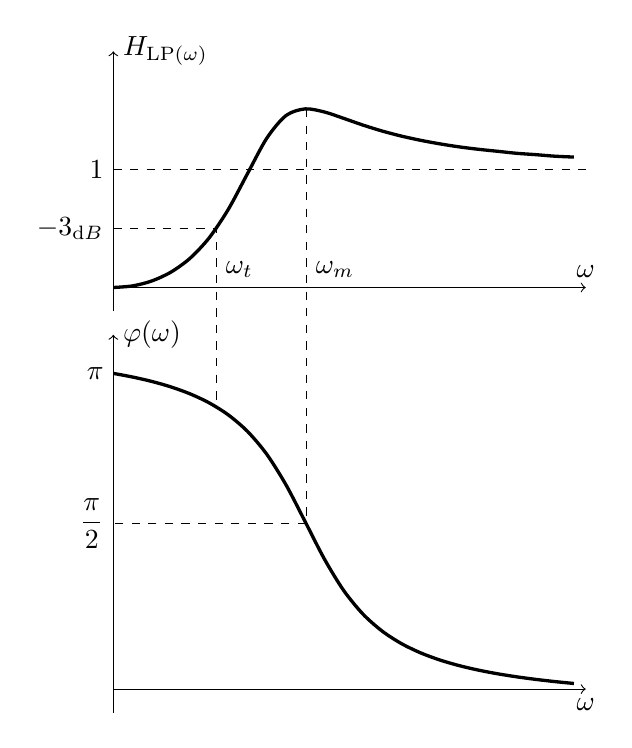
\begin{tikzpicture}[scale=1.5]
    \draw[->](0,1.8)--(0,4)node[right]{$H_{\mathrm{LP}(\omega)}$};
    \draw[->](0,2)--(4,2)node[above]{$\omega$};
    \draw[very thick, smooth, domain=0:3.9]plot(\x,{2+2*((\x)^2)*((4-2*(\x)^2)^2+(2*\x)^2)^(-0.5)});
    \draw[dashed](0,3)node[left]{$1$}--(4,3);
    \draw[dashed](1.633,3.512)--(1.633,2)node[above right]{$\omega_m$}--(1.633,0)--(0,0)node[left]{$\displaystyle\frac{\pi}{2}$};
    \draw[->](0,-1.6)--(0,1.6)node[right]{$\varphi(\omega)$};
    \draw[very thick, smooth, domain=0:3.9]plot(\x,{pi/180*atan(-2*(\x-1.633))});
    \draw[->](0,-1.4)--(4,-1.4)node[below]{$\omega$};
    \node[left]at(0,1.274){$\pi$};
    \draw[dashed](0,2.5)node[left]{$-3_{\mathrm{d}B}$}--(0.871,2.5)--(0.871,2)node[above right]{$\omega_t$}--(0.871,0.99);
\end{tikzpicture}
\end{document}